% Gere o PDF com o comando pdflatex, e o SVG com o comando
%
%  $ inkscape -l fig.svg source.tex
\documentclass{standalone}
\usepackage{tikz}

\begin{document}

    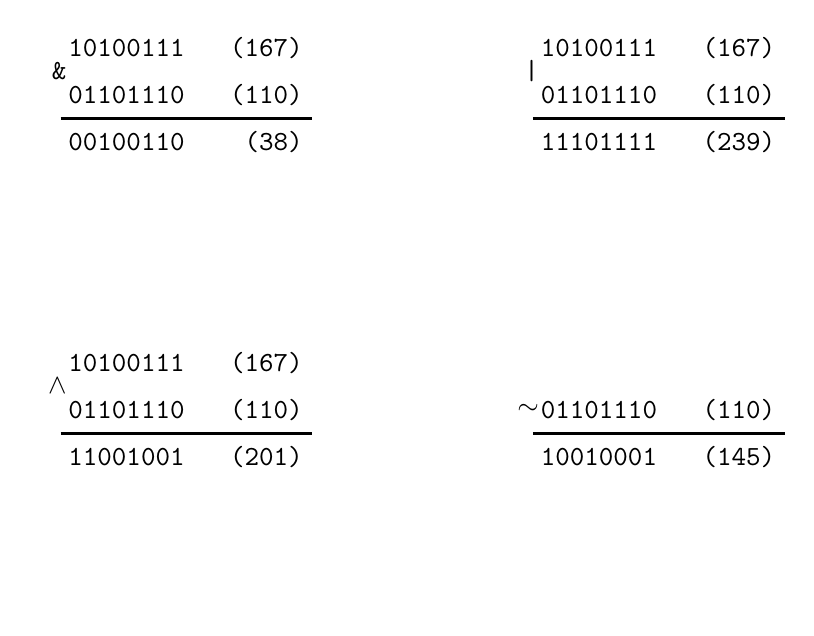
\begin{tikzpicture}
        \begin{scope}
            \node[opacity=0] at (0, 0) { };

            \node[anchor=east] at (2, 3) {  \texttt{10100111} };
            \node[anchor=east] at (3.5, 3) {  \texttt{(167)} };
            \node[anchor=east] at (2, 2.4) {  \texttt{01101110} };
            \node[anchor=east] at (3.5, 2.4) {  \texttt{(110)} };
            \node[anchor=east] at (0.5, 2.7) {  \texttt{\&} };

            \draw[thick] (0.3, 2.1) -- (3.5, 2.1);

            \node[anchor=east] at (2, 1.8) {  \texttt{00100110} };
            \node[anchor=east] at (3.5, 1.8) {  \texttt{(38)} };
        \end{scope}

        \begin{scope}[shift={(6,0)}]
            \node[opacity=0] at (0, 0) { };

            \node[anchor=east] at (2, 3) {  \texttt{10100111} };
            \node[anchor=east] at (3.5, 3) {  \texttt{(167)} };
            \node[anchor=east] at (2, 2.4) {  \texttt{01101110} };
            \node[anchor=east] at (3.5, 2.4) {  \texttt{(110)} };
            \node[anchor=east] at (0.5, 2.7) {  \texttt{|} };

            \draw[thick] (0.3, 2.1) -- (3.5, 2.1);

            \node[anchor=east] at (2, 1.8) {  \texttt{11101111} };
            \node[anchor=east] at (3.5, 1.8) {  \texttt{(239)} };
        \end{scope}

        \begin{scope}[shift={(0,-4)}]
            \node[opacity=0] at (0, 0) { };

            \node[anchor=east] at (2, 3) {  \texttt{10100111} };
            \node[anchor=east] at (3.5, 3) {  \texttt{(167)} };
            \node[anchor=east] at (2, 2.4) {  \texttt{01101110} };
            \node[anchor=east] at (3.5, 2.4) {  \texttt{(110)} };
            \node[anchor=east] at (0.5, 2.7) {  $\land$ };

            \draw[thick] (0.3, 2.1) -- (3.5, 2.1);

            \node[anchor=east] at (2, 1.8) {  \texttt{11001001} };
            \node[anchor=east] at (3.5, 1.8) {  \texttt{(201)} };
        \end{scope}

        \begin{scope}[shift={(6,-4)}]
            \node[opacity=0] at (0, 0) { };

            \node[anchor=east] at (2, 2.4) {  \texttt{01101110} };
            \node[anchor=east] at (3.5, 2.4) {  \texttt{(110)} };
            \node[anchor=east] at (0.5, 2.4) {  $\sim$ };

            \draw[thick] (0.3, 2.1) -- (3.5, 2.1);

            \node[anchor=east] at (2, 1.8) {  \texttt{10010001} };
            \node[anchor=east] at (3.5, 1.8) {  \texttt{(145)} };
        \end{scope}

    \end{tikzpicture}

\end{document}
